\chapter{Architecture et conception}

\section*{Introduction}
\addcontentsline{toc}{section}{Introduction}
    \par Le troisième chapitre explore l'architecture du projet et sa étude conceptuelle. Nous justifions notre choix d'une architecture en couches et détaillons notre modèle de données conceptuel basé sur le modèle entité-association, offrant ainsi une base solide pour notre solution.

\section{Étude architecturale}
\par Le choix de l'architecture d'une application revêt une importance capitale dans le processus de conception d'un projet. 
Le choix de l'architecture détermine comment les diverses parties de l'application interagiront pour atteindre les objectifs fixés.
Dans notre projet, nous avons délibérément opté pour \textbf{une architecture micro-services}, une décision dictée par des critères spécifiques qui s'accordent parfaitement avec les exigences de notre projet.
Dans cette section, nous explorerons en détail les raisons de notre choix.
\subsection{Justification du choix de l'architecture en couches}
\begin{itemize}
        \item \textbf{Séparation des responsabilités: }L'architecture en couches est réputée pour sa capacité à réaliser une distinction claire des responsabilités \cite{sep}. 
        \par Dans notre projet, il est impératif de maintenir une séparation nette entre la couche d'interface utilisateur, la couche de logique métier, la couche d'accès aux données et la couche d'infrastructure. 
        \par Cette distinction des responsabilités s'avère essentielle pour gérer efficacement les multiples facettes du projet, de la collecte de données à la visualisation des résultats.
        \item \textbf{Modularité et réutilisation: }L'architecture en couches favorise la modularité, ce qui signifie que chaque couche peut être conçue comme un composant indépendant. \cite{module}
        \par Cette modularité est un atout majeur pour notre projet, car elle simplifie le développement et la maintenance de chaque couche de manière indépendante. Cela facilite également la réutilisation de composants dans d'autres projets à venir. 
        \item \textbf{Facilité de maintenance et d'évolution:} L'architecture en couches facilite la maintenance continue et l'évolution du projet. En cas de modifications nécessaires dans une couche spécifique, elles peuvent être apportées sans perturber les autres couches. Par exemple, si de nouvelles sources de données doivent être intégrées, cela peut être géré au niveau de la couche d'accès aux données sans affecter la logique métier ou l'interface utilisateur.\cite{facilite} Cette capacité à évoluer rapidement est cruciale pour notre projet, étant donné qu'il évolue dans un environnement en constante mutation.
\end{itemize}
\par En conclusion, l'architecture en couches s'impose comme le choix idéal pour notre projet en raison de sa capacité à séparer les responsabilités, à encourager la modularité et à faciliter la maintenance. Elle fournit une base solide pour le développement d'une solution d'analyse de performance robuste et évolutive. Cette décision architecturale renforce notre aptitude à atteindre nos objectifs dans un environnement professionnel en constante évolution.
\subsection{Architecture logique} 
\par Cette section explorera en détail l'architecture du projet. Elle mettra en lumière les différentes couches fonctionnelles qui la composent et expliquera comment ces composantes interagissent pour fournir une expérience utilisateur fluide et des analyses de performance précises. 
\par L'architecture logique constitue le socle sur lequel repose la réalisation de l'objectif du projet et ceci est illustrée par la figure \textbf{\ref{fig:arch_log}} suivante:
%code image
        \begin{figure}[H]
        \centering
        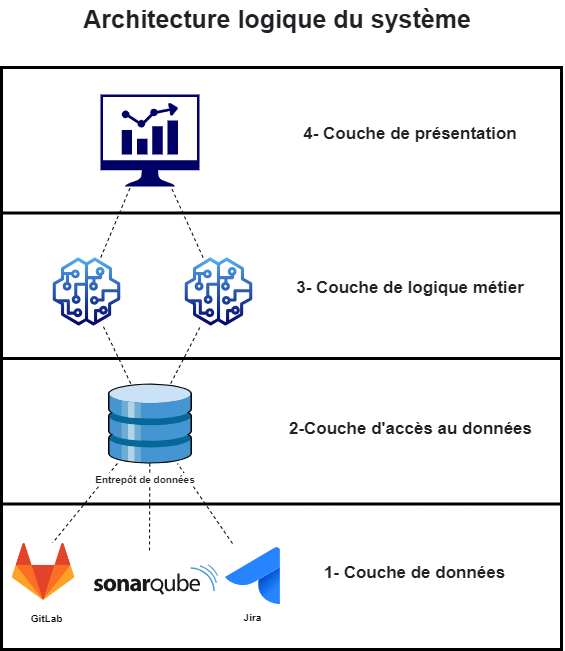
\includegraphics[width = 12cm , height=10cm]{img/techno/archi_log.png}
        \caption{Architecture logique du projet}
        \label{fig:arch_log}
        \end{figure}
        %fin
    \par Nous plongerons dans les diverses couches de l'architecture logique, décrivant leurs rôles et expliquant comment elles contribuent à l'ensemble du projet. Cela donnera un aperçu clair de la manière dont les données sont collectées, transformées, analysées, et enfin affichées à travers un tableau de bord convivial.
    \begin{enumerate}

        \item[1.] \textbf{Couche de données: } 
                \begin{itemize}
                \item Cette composante supervise l'extraction de données provenant de diverses sources, comme Jira, Gitlab, et SonarQube.
                \item Elle garantit une transformation et une intégration harmonieuse des données pour une analyse ultérieure.
                \item Cette couche s'occupe des tâches d'automatisation et de collecte de données.
            \end{itemize}
            
         \item[2.] \textbf{Couche d'accès aux données: }
                \begin{itemize}
                \item Cette couche stocke de manière centralisée les données nécessaires à l'analyse de la performance de l'équipe.
                \item Elle veille à la cohérence des données, à la gestion sécurisée des informations, et à un accès fiable aux données.
                \item Les bases de données relationnelles stockent données brutes et résultats analytiques.
            \end{itemize}
            
        \item[3.] \textbf{Couche de logique métier: }
                \begin{itemize}
                \item Cette couche assure la gestion de la logique métier de l'application en collectant, traitant, et examinant les données.
                \item Elle interagit avec l'interface utilisateur pour fournir des informations pertinentes, des fonctionnalités d'analyse, et des résultats.
                \item Dans cette couche, les algorithmes d'analyse, de prévision, et de relation sont mis en place pour extraire des informations significatives à partir des données non transformées.
            \end{itemize}
            
        \item[4.] \textbf{Couche de Présentation:}
            \begin{itemize}
                \item Cette couche représente la facette visible de votre application, où les utilisateurs engagent avec le tableau de bord.
                \item Elle offre une expérience utilisateur conviviale et interactive pour la visualisation des données de performance et des résultats d'analyse.
                \item Des graphiques, des tableaux de bord personnalisés, et des fonctionnalités conviviales sont élaborés ici pour une expérience utilisateur optimale.
            \end{itemize}
    \end{enumerate}
    \subsection{Architecture physique}
    \par L'architecture physique d'un projet constitue la matérialisation concrète de son architecture logique. Elle se consacre aux aspects matériels et aux ressources nécessaires pour assurer le bon fonctionnement de l'application\cite{archi_phy}. Dans notre cas, l'architecture physique revêt une importance cruciale pour garantir une exécution sans heurts de la solution.

    \par Cette section se plonge dans les subtilités de l'architecture matérielle, intégrant diverses technologies et composants essentiels pour maintenir une performance optimale. Ces éléments techniques sont soigneusement élaborés afin de fonctionner de manière fluide et efficace, permettant ainsi la collecte, le traitement, le stockage et la présentation optimisés des données.
\par la figure \textbf{\ref{fig:arch_phy}} suivante illustre l'architecture adopté dans ce projet : 
%code image
        \begin{figure}[H]
        \centering
        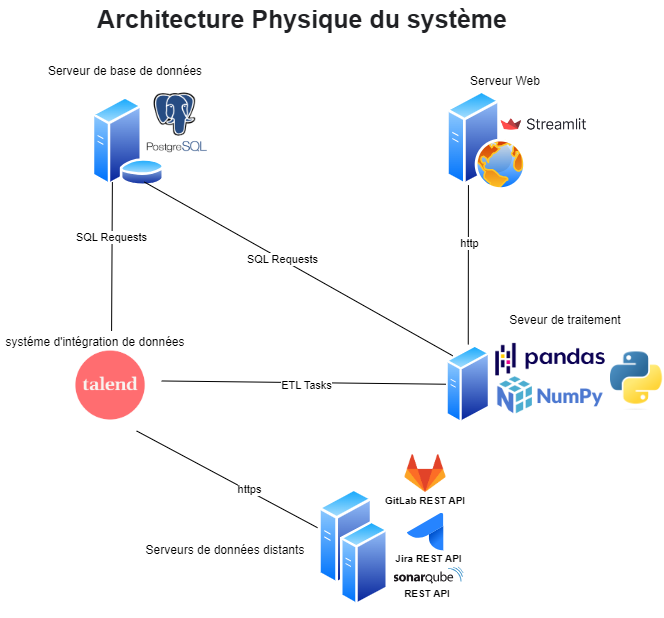
\includegraphics[width = 17cm , height=15cm]{img/techno/archi_phy.png}
        \caption{Architecture logique}
        \label{fig:arch_phy}
        \end{figure}
        %fin
        \par Notre architecture physique est composée de plusieurs éléments essentiels qui travaillent en tandem pour permettre la collecte, le traitement, le stockage et la présentation des données de manière optimale. Voici un aperçu détaillé de ces composants :
        \begin{enumerate}
            \item[1-] \textbf{Serveur de présentation : } 
            \par Ce serveur est responsable de l'affichage du tableau de bord à l'interface utilisateur. Il utilise la technologie Streamlit, qui permet de créer des interfaces interactives en Python. Les utilisateurs interagissent avec cette interface pour visualiser les données et les performances de l'équipe Avaxia.
            \item [2-] \textbf{Serveur de Traitement :} 
            \par Ce serveur assume la lourde tâche de l'exécution des traitements de données. Il repose sur Python, accompagné des bibliothèques NumPy et Pandas, pour effectuer les opérations statistiques et de calcul sur les données. Il est essentiel pour la collecte, le nettoyage, l'analyse des corrélations et la prédiction des performances futures.
            \item[3-]  \textbf{Serveur de Base de Données: }
            \par Ce serveur stocke de manière centralisée toutes les données nécessaires à l'analyse de la performance de l'équipe Avaxia. L'utilisation de PostgreSQL garantit la cohérence des données, leur facilité d'accès et leur gestion sécurisée.

            \item[4-] \textbf{Serveurs de Données Distants:}
            \par Ces serveurs sont utilisés pour l'accès aux API externes, notamment les API de Jira, Gitlab et SonarQube. Ils sont essentiels pour extraire des données détaillées telles que les informations sur les tickets, les commits de code et les mesures de performance de l'équipe Avaxia.
        \end{enumerate}
    \par En conclusion, L'architecture physique de notre projet crée une infrastructure solide qui permet une gestion efficace des données, du traitement à la présentation, offrant ainsi à l'équipe Avaxia une vue complète et pratique de sa performance. Chacun des composants est interconnecté pour assurer un fonctionnement harmonieux du système.

\section{Étude conceptuelle}
\par Dans cette section on va s'intéresser à la modélisation de notre projet à l'aide des différents modelés et diagrammes qui vont nous permettre de mieux comprendre le flux de travail ainsi la nature des données qui circule dans notre système.
\subsection{Modèle entité-association}
\par Le modèle entité-association, permet d’avoir une représentation graphique de la base de données, ce qui simplifie la compréhension. La version simplifiée de ce modèle est plus compréhensible mais n'inclut pas toutes les caractéristiques d'une table de données, dont notamment les liens entre les entités \cite{E_A}. 
\par la figure \textbf{\ref{fig:e_a}} qui suit représente le modèle entité association de notre système: 
     %code image
        \begin{figure}[H]
        \centering
        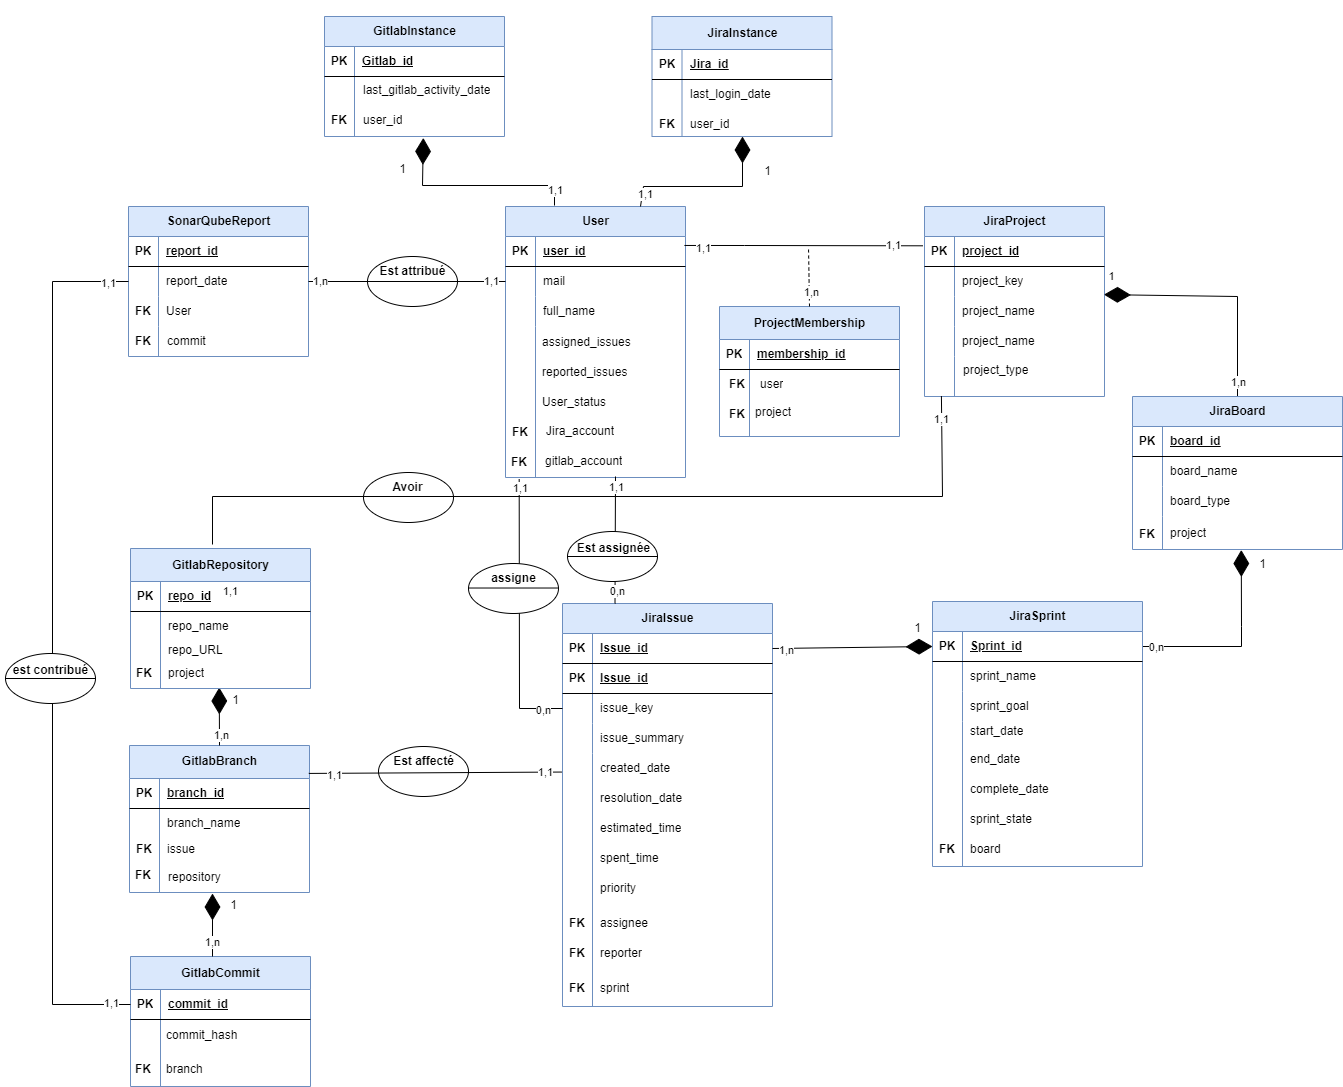
\includegraphics[width = 17cm , height=14cm]{img/conception/E_a.png}
        \caption{Modèle entité-association}
        \label{fig:e_a}
        \end{figure}
    %fin
    \subsection{Description détaillée des entités et des associations}
    Dans cette partie on va focaliser sur les différents entités et leurs associations qui construisent notre base de données globale dont on a modélisé précédemment.
    \begin{itemize}
        \item \textbf{Entité JiraInstance :} cette entité représente une instance GitLab liée à un utilisateur.
        Le tableau \textbf{3.1} suivant représente la liste de ces attributs: 

            \begin{center}   
                \begin{longtable}{|p{3cm}|p{11cm}|p{2cm}|}
                    \caption {Description de l'entité "JiraInstance"} \\
                    \hline
                    \rowcolor{blue!18}\textbf{\large{Nom d'attribut}} & \textbf{\large{Description}} & \textbf{\large{Type}} \\
                    \hline
                    ID&  Identifiant unique de l'instance Jira&  Varchar\\\hline
                    last\_login\_date& Date de la dernière connexion& Datetime\\\hline

                \end{longtable}
                

            \end{center}
            \vspace{-1cm}
        \item \textbf{Entité GitlabInstance :}cette entité représente une instance Jira liée à un utilisateur.
        Le tableau \textbf{3.2} suivant représente la liste de ces attributs: 
        \begin{center}   
                \begin{longtable}{|p{5cm}|p{9cm}|p{2cm}|}
                    \caption {Description de l'entité "GitlabInstance"} \\
                    \hline
                    \rowcolor{blue!18}\textbf{\large{Nom d'attribut}} & \textbf{\large{Description}} & \textbf{\large{Type}} \\
                    \hline
                    ID&  Identifiant unique de l'instance Gitlab&  Varchar\\\hline
                    last\_gitlab\_activity\_date& Date de la dernière activité en Gitlab& Datetime\\\hline

                \end{longtable}

            \end{center}
        \vspace{-1cm}
        \item \textbf{Entité User:} cette entité stocke des informations sur les utilisateurs du système, y compris leurs comptes Jira et GitLab.
        Le tableau \textbf{3.3} suivant représente la liste de ces attributs:
        \begin{center}   
                \begin{longtable}{|p{3cm}|p{11cm}|p{2cm}|}
                    \caption {Description de l'entité "User"} \\
                    \hline
                    \rowcolor{blue!18}\textbf{\large{Nom d'attribut}} & \textbf{\large{Description}} & \textbf{\large{Type}} \\
                    \hline
                    user\_id& Identifiant unique de l'utilisateur&  Entier\\\hline
                    mail&Adresse e-mail de l'utilisateur& 5 Varchar\\\hline
                    full\_name& Nom complet de l'utilisateur& Varchar\\\hline
                    assigned\_issues& Nombre d'issues attribuées à l'utilisateur&\ Entier\\\hline
                    reported\_issues&Nombre d'issues signalées par l'utilisateur&\ Entier\\\hline
                    user\_status & Statut de l'utilisateur&\ Varchar\\\hline
                    jira\_account  & Identifiant du compte Jira &\ Varchar\\\hline
                    gitlab\_account  &  Identifiant du compte GitLab&\ Varchar\\\hline


                \end{longtable}
            
            \end{center}
            \vspace{-1cm}
        \item \textbf{Entité JiraProject:} cette entité représente un projet Jira et ses informations.
        Le tableau \textbf{3.4} suivant représente la liste de ces attributs:
        \begin{center}   
                \begin{longtable}{|p{3cm}|p{11cm}|p{2cm}|}
                    \caption {Description de l'entité "JiraProject"} \\
                    \hline
                    \rowcolor{blue!18}\textbf{\large{Nom d'attribut}} & \textbf{\large{Description}} & \textbf{\large{Type}} \\
                    \hline
                    project\_id& Identifiant unique du projet Jira.&  Entier\\\hline
                    project\_key& Clé du projet Jira& Varchar\\\hline 
                    project\_name&Nom du projet & Varchar\\\hline
                    project\_type& Type de projet &Varchar\\\hline
                    number\_issues&Nombre d'issues associées au projet &Entier \\\hline
                                        

                \end{longtable}
               
            \end{center}
            \vspace{-1cm}
        \item \textbf{Entité ProjectMembership:} cette entité représente l'appartenance d'un utilisateur à un projet Jira.
        Le tableau \textbf{3.5} suivant représente la liste de ces attributs:
        \begin{center}   
                \begin{longtable}{|p{3cm}|p{11cm}|p{2cm}|}
                    \caption {Description de l'entité "ProjectMembership"} \\
                    \hline
                    \rowcolor{blue!18}\textbf{\large{Nom d'attribut}} & \textbf{\large{Description}} & \textbf{\large{Type}} \\
                    \hline
                    membership\_id& Identifiant unique de l'appartenance au projet &  Entier\\\hline
                    user& Identifiant de l'utilisateur associé à l'appartenance& Entier\\\hline
                    project& Identifiant du projet Jira associé&\ Entier\\\hline
                                        

                \end{longtable}
               
        \end{center}
        \vspace{-1cm}
        \item \textbf{Entité JiraBoard:} cette entité représente un tableau (board) dans Jira et ses caractéristiques.
        Le tableau \textbf{3.6} suivant représente la liste de ces attributs:
        \begin{center}   
                \begin{longtable}{|p{3cm}|p{11cm}|p{2cm}|}
                    \caption {Description de l'entité "JiraBoard"} \\
                    \hline
                    \rowcolor{blue!18}\textbf{\large{Nom d'attribut}} & \textbf{\large{Description}} & \textbf{\large{Type}} \\
                    \hline
                    board\_id&  Identifiant unique du tableau Jira &  Entier\\\hline
                    board\_name& Nom du tableau& Varchar\\\hline
                    board\_type& Type de tableau &\ Varchar\\\hline
                    project& Projet associé au tableau&\ Entier\\\hline
                                    

                \end{longtable}
               
        \end{center}
        \vspace{-1cm}
        \item \textbf{Entité JiraSprint:} cette entité stocke des informations sur les sprints dans Jira.
        Le tableau \textbf{3.7} suivant représente la liste de ces attributs:
        \begin{center}   
                \begin{longtable}{|p{3cm}|p{11cm}|p{2cm}|}
                    \caption {Description de l'entité "JiraSprint"} \\
                    \hline
                    \rowcolor{blue!18}\textbf{\large{Nom d'attribut}} & \textbf{\large{Description}} & \textbf{\large{Type}} \\
                    \hline
                    sprint\_id&  Identifiant unique du tableau Jira &  Entier\\\hline
                    sprint\_name& Nom du tableau& Varchar\\\hline
                    sprint\_goal& Type de tableau &\ Texte\\\hline
                    start\_date& Date de début du sprint&\ Datetime\\\hline
                    end\_date& Date de fin du sprint&\ Datetime\\\hline
                    complete\_date& Date de clôture du sprint&\ Datetime\\\hline
                    sprint\_state & État du sprint &\ Varchar\\\hline
                    board&Tableau Jira  au quelle le sprint est associé &Entier\\\hline
                                   
                \end{longtable}
        \end{center}
        \vspace{-1cm}
        \item \textbf{Entité JiraIssue:}cette entité stocke des informations sur les issues Jira.
        Le tableau \textbf{3.8} suivant représente la liste de ces attributs:
        \begin{center}   
                \begin{longtable}{|p{3cm}|p{11cm}|p{2cm}|}
                    \caption {Description de l'entité "JiraIssue"} \\
                    \hline
                    \rowcolor{blue!18}\textbf{\large{Nom d'attribut}} & \textbf{\large{Description}} & \textbf{\large{Type}} \\
                    \hline
                    issue\_id&   Identifiant unique de l'issue Jira&  Entier\\\hline
                    issue\_key&Clé de l'issue Jira& Varchar\\\hline
                    issue\_summary& Résumé de l'issue &\ Texte\\\hline
                    creation\_date& Date de création de l'issue&\ Datetime\\\hline
                    updated\_date& Date de fin de l'issue&\ Datetime\\\hline
                    resolution\_date&  Date de résolution de l'issue &\ Datetime\\\hline
                    issue\_status & Statut de l'issue &\ Varchar\\\hline
                    issue\_type & Type de l'issue&\ Varchar\\\hline
                    estimated\_time & Temps estimé pour l'issue(heurs)&\ Entier\\\hline
                    spent\_time &  Temps passé sur l'issue(heurs)&\ Entier\\\hline
                    priority&Priorité de l'issue&Varchar\\\hline
                    assignee&Identifiant de l'utilisateur assigné à l'issue&Varchar\\\hline
                    reporter& Identifiant de l'utilisateur ayant signalé l'issue &Varchar\\\hline
                    sprint&Identifiant du sprint associé à l'issue&Entier\\\hline
                                   

                \end{longtable}
        \end{center}
        \vspace{-1cm}
        \item \textbf{Entité GitlabRepository:} cette entité représente un dépôt GitLab associé à un projet Jira.
        Le tableau \textbf{3.9} suivant représente la liste de ces attributs:
        \begin{center}   
                \begin{longtable}{|p{3cm}|p{11cm}|p{2cm}|}
                    \caption {Description de l'entité "GitlabRepository"} \\
                    \hline
                    \rowcolor{blue!18}\textbf{\large{Nom d'attribut}} & \textbf{\large{Description}} & \textbf{\large{Type}} \\
                    \hline
                    repo\_id& Identifiant unique du dépôt&  Entier\\\hline
                    repo\_name& Nom du dépôt& Varchar\\\hline
                    repo\_URL& URL du dépôt &\ Varchar\\\hline
                    project& Identifiant du projet associé à cet dépôt&\ Entier\\\hline
                               

                \end{longtable}
        \end{center}
        \vspace{-1cm}
        \item \textbf{Entité GitlabBranch:}Cette entité représente une branche GitLab liée à une issue Jira.
        Le tableau \textbf{3.10} suivant représente la liste de ces attributs:
        \begin{center}   
                \begin{longtable}{|p{3cm}|p{11cm}|p{2cm}|}
                    \caption {Description de l'entité "GitlabBranch"} \\
                    \hline
                    \rowcolor{blue!18}\textbf{\large{Nom d'attribut}} & \textbf{\large{Description}} & \textbf{\large{Type}} \\
                    \hline
                    branch\_id& Identifiant unique du branche&  Entier\\\hline
                    branch\_name& Nom du branche& Varchar\\\hline
                    issue& Identifiant de l'issue associé à cette branche &\ Varchar\\\hline
                    repository & Identifiant du dépôt associé à cette branche&\ Entier\\\hline
                
                \end{longtable}
        \end{center}
        \vspace{-1cm}
        \item \textbf{Entité GitlabCommit:}Cette entité stocke des informations sur les commits GitLab, en lien avec une branche spécifique.
        Le tableau \textbf{3.11} suivant représente la liste de ces attributs:
        \begin{center}   
                \begin{longtable}{|p{3cm}|p{11cm}|p{2cm}|}
                    \caption {Description de l'entité "GitlabCommit"} \\
                    \hline
                    \rowcolor{blue!18}\textbf{\large{Nom d'attribut}} & \textbf{\large{Description}} & \textbf{\large{Type}} \\
                    \hline
                    commit\_id& Identifiant unique du branche&  Entier\\\hline
                    commit\_hash& Nom du branche& Varchar\\\hline
                    branch& Identifiant du projet associé à ce commit&\ Entier\\\hline
              

                \end{longtable}
        \end{center}
        \vspace{-1cm}
        \item \textbf{Entité SonarqubeReport:}Cette entité contient des rapports de SonarQube liés à des commits GitLab.
        Le tableau \textbf{3.12} suivant représente la liste de ces attributs:
        \begin{center}   
                \begin{longtable}{|p{3cm}|p{11cm}|p{2cm}|}
                    \caption {Description de l'entité "SonarqubeReport"} \\
                    \hline
                    \rowcolor{blue!18}\textbf{\large{Nom d'attribut}} & \textbf{\large{Description}} & \textbf{\large{Type}} \\
                    \hline
                    report\_id& Identifiant unique du rapport SonarQube &  Entier\\\hline
                    report\_date& Date d'élaboration du rapport& Varchar\\\hline
                    commit& Identifiant du commit associé à ce rapport &\ Varchar\\\hline
                    user& Identifiant de l'utilisateur associé à ce rapport&\ Entier\\\hline
                    

                \end{longtable}
        \end{center}

    \end{itemize}
    
\section*{Conclusion}
\addcontentsline{toc}{section}{Conclusion }

    Ce chapitre a établi les bases pour la mise en œuvre technique de notre projet. Les choix architecturaux et conceptuels s'avèrent essentiels pour assurer la stabilité et la performance de notre solution. Dans le prochain chapitre, nous plongerons dans la réalisation concrète de notre projet.